\documentclass[11pt, oneside]{article}
\usepackage[T1]{fontenc}
\usepackage{titling, geometry, hyperref, fancyhdr, algorithm, enumitem}
\usepackage{amsmath, amssymb, amsthm}              % mathematical packages
\usepackage{graphicx, subcaption, wrapfig}         % images
\usepackage{textcomp, CJKutf8}                     % misc. text formatting
\usepackage{tikz, pgfplots, tikz-network}          % plots and graphs
\usepackage[noend]{algpseudocode}                  % algorithm psuedocode
\usepackage[cache=true]{minted}                    % source code
\usepackage[style=numeric, sorting=none]{biblatex} % bibliography
\geometry{a4paper}

\hypersetup{
  colorlinks=true,
  urlcolor=cyan,
  linkcolor=black
}

\setminted[]{
  linenos=false,
  breaklines=true,
  encoding=utf8,
  fontsize=\small,
  frame=topline,
  framesep=2mm
}

% https://tex.stackexchange.com/questions/343494/minted-red-box-around-greek-characters
\makeatletter
\AtBeginEnvironment{minted}{\dontdofcolorbox}
\def\dontdofcolorbox{\renewcommand\fcolorbox[4][]{##4}}
\makeatother

\newcommand{\emphasis}[1]{\textbf{\textit{#1}}}
\graphicspath{{./images/}}
\addbibresource{ref.bib}

\title{Hog Contest Postmortem Analysis}
\author{Stephen Huan, ``Mikoto Misaka and the Tree Diagram'' \\
\href{https://hog-contest.cs61a.org/winners}{2\textsuperscript{nd} place summer 2020}}
\date{July 13, 2020}

\begin{document}
\maketitle
\tableofcontents

\newpage

\section{Introduction}

Clicking on entries in the table of contents 
will bring you to the corresponding section. 
URLs are colored \textcolor{cyan}{blue} and 
important words are \emphasis{emphasized}.
If either of these style choices are hard to read,
consider modifying the \LaTeX \ source file
(urlcolor is defined on line 14 and the emphasis command is defined on line 33).

Code is formatted like this:
\begin{minted}[label=code example]{python}
print("Hello, world!")
\end{minted}

Python 3 is used in all code examples, although 
the actual code is ran with \href{https://www.pypy.org/}{PyPy}, an alternative
implementation of the Python interpreter that runs roughly 12x faster 
than standard Python. PyPy works with all standard libraries,
and is in general a nearly drop-in replacement for standard Python.
Considering some scripts run for nearly 10 minutes, installing 
PyPy is highly recommended.

Personally, I would recommended re-writing everything in C++, a low-level
compiled language that adds functionality onto C. Considering CS61A
is a Python class, that might be unrealistic, but C++ is nearly 
100x faster than Python in some cases.

\subsection{Definitions}

\href{https://cs61a.org/proj/hog/}{Hog} is a dice-based game with a variety of rules.
The \href{https://cs61a.org/proj/hog_contest/}{Hog contest} is the problem
of playing the game as well as possible, where playing the game ``well''
means to maximize \emphasis{win rate}. Win rate can be thought of 
as the percentage of games you would win playing against an opponent 
over and over again, where the number of games you play is infinite.
A \emphasis{game} can be thought of as a series of \emphasis{states},
where each state contains all the information about the game's current position.
At each state, a player makes a move, which moves the game from the current state
to different state. The game terminates at a final state,
where the outcome of the game is certain (win or loss).
The outcome of a game is known as \emphasis{utility}, because
it is what both players wants to optimize.
Under this abstraction of games, each game is essentially a decision tree
that propagates downwards until the leaves are final states, where 
the game is either won or lost (technically speaking, each game is a 
directed acyclic graph, but the tree visual is clearer).
For a concrete example, consider the game of chess.
The game starts off in the initial state of the initial chessboard,
and now the white player has a variety of moves available to them.
Each move they can make is imagined as a child of the initial chessboard
in the tree. Then, the children of the children of the initial state 
are the possible boards resulting from black moving. This branching pattern
repeats until we reach leaf nodes, which in chess are boards where either
one player is in checkmate or there is a draw.
Chess and Hog are also \emphasis{zero-sum}, because any gain in utility 
for a player is equivalent to a loss in utility for the opponent.

\subsection{Approaches}

The fundamental question is, under what framework can gameplay be considered optimal?
In chess, one simple algorithm is \emphasis{minimax}. Imagine a leaf node in chess.
Since it is known whether or not a player won, lost, or tied, that node
has a defined utility. Take a node \( u \) whose children are all leaf nodes.
The optimal move at \( u \) is obviously just the move which gives the best
leaf node, and \( u \)'s utility is the utility of the best leaf node.
This defines utility for nodes that are one move away from a leaf node.
Repeating this recursive definition of utility, one computes the 
best possible move for all chessboards by propagating utility 
in this bottom-up manner (leaves to root). 
Since chess has an absurd number of possible boards,
in practice no computer could run fast enough to explore all possible boards,
and instead the search has to be cut off at a certain depth 
and the utility of the cut-off ``leaf'' nodes measured with a \emphasis{heuristic}
(a function which tries to approximate the real utility at a node).
Monte-Carlo Tree Search (MCTS) essentially replaces minimax's heuristic with 
gameplay simulation at each node, and was notably used by Google
to create the strongest Go player ever created, 
\href{https://deepmind.com/blog/article/alphazero-shedding-new-light-grand-games-chess-shogi-and-go}{AlphaZero}.

Both algorithms could theoretically play chess, Go, tic-tac-toe,
etc. optimally given enough computational time. 
Chess and Hog seem similar based off our abstract definition of a game,
so one might think it would simple to apply minimax or MCTS to Hog;
however, there are two key differences: dependence on opponent play and information.

For an example of the former, consider rock-paper-scissors (RPS).
The optimal strategy is dependent on the opponent's strategy:
if the opponent always plays rock then 
the optimal strategy is to always play paper.
Chess does not have this dependency: the assumption is that the opponent 
plays optimally (in accordance to the same bottom-up algorithm).
If the opponent plays sub-optimally, 
then the player can take advantage of that mistake. 
Put simply, \textit{any deviation from the optimal strategy is a mistake}.

The second key assumption is that there is 
an one-to-one correspondence between game states 
and the information available to each player. 
The optimal move at any state can be determined by just looking 
at the chessboard, there is no secret information.
This is different for a game like Poker.
In Poker, if one knows the cards of their opponents, they have a huge advantage.
There is hidden information, so the game is \emphasis{partially observable}.
In these sorts of games, rather than an absolute state being associated with 
each node in the tree, there is an \emphasis{information set}
which represents the variety of possible states that a player could be at.

In Hog, the feral hogs rule moves the game from a perfect information
game like chess to a partially observable game like Poker.
Since a strategy does not know the change in scores for them or their opponent,
they cannot reliably predict whether the feral hogs rule applies or not. 
At this point I want to make a distinction between stochasticity and uncertainty.
A \emphasis{stochastic} game is just any game with random elements
whose probability distributions are known \textit{a priori}.
Hog is stochastic because rolling the dice is an inherently random action.
A game being stochastic does not disqualify minimax, however.
A stochastic game can be thought of as a non-stochastic game,
except instead of a move's utility being the utility of the state 
that it transitions to, a move's utility is the expected value utility
over all the possible states that performing the move could go to.
An \emphasis{uncertain} game, on the other hand, is a game with random elements 
whose probability distributions are known \textit{a posteriori}.
Since the probability of a certain change in score is dependent on
opponent strategy, it is impossible to determine a probability distribution
of the changes in score (as compared to dice rolls, whose probability 
distributions are known ahead of time and are independent of strategy).

This causes a fundamental problem for minimax and MCTS.
The proper, mathematical concept of a solution for these types of games
is the \emphasis{Nash equilibrium}. The Nash equilibrium is defined 
as a pair of strategies such that unilateral deviation from 
the Nash equilibrium cannot improve play. 
An implication is that a strategy where the opponent
is indifferent to each action, i.e. the expected value of each of their actions
is the same, is also a Nash equilibrium. In this solution definition,
a \emphasis{strategy} is a mapping between information sets and 
the probability of performing each possible action.
A \emphasis{pure strategy} is one where 
the probability of playing a particular action is 1, 
and the probability of playing all other actions is 0.
A \emphasis{mixed strategy} is a non-pure strategy.
In chess, each information set is just the chessboard,
since there is no hidden information.
The strategy would define for each chessboard the probability of playing
each possible action, and in chess it is possible to play optimally 
with a pure strategy (where the move for a particular board is fixed).

An algorithm for calculating the Nash equilibrium is 
Counterfactual Regret Minimization (CFR).
\footnote{See the \href{http://modelai.gettysburg.edu/2013/cfr/cfr.pdf}{guide},
or my explanation 
\href{https://github.com/stephen-huan/sct-lectures/blob/master/ml/gametheory/lecture.pdf}{here}.}
Implementation is beyond the scope of this analysis.
\footnote{My Python implementation can be found 
\href{https://github.com/stephen-huan/Counterfactual-Regret-Minimization}{here}.}
I attempted to implement Fixed-Strategy Iteration CFR and apply it to Hog, 
but it took too long to run and it was too late into the contest.

Instead, I will show the approach I actually used: a recursive dynamic programming
algorithm styled after minimax, and the final improvement: 
a heuristical technique to estimate the distribution of the changes in score
that determine the feral hogs rule.

\newpage

\section{Dynamic Programming}

\emphasis{Dynamic programming} (DP) is a programming technique that takes advantage
of repetitive structure in the solution of a problem to speed up calculation. 
\footnote{See chapter 15 of \textit{Introduction to Algorithms},
the classic MIT book by Cormen, Leiserson, Rivest, and Stein
(also named CLRS after the authors' initials) for a more thorough treatment.}
Dynamic programming will be used two-fold: to compute the probability distribution
of dice rolls, and to compute the optimal move for each information set,
ignoring the feral hogs rule.

One useful thing to know would be the probability distribution of dice rolls.
For example, if I roll 6 dice, what are the chances that the sum of rolls is 10?
Will rolling 7 dice improve my probability of getting a 10?
We call the sum of rolls \emphasis{deltas}, 
since they represent the change in score for the turn.
The distribution we will actually calculate
is the probability mass function (PMF), or the discrete equivalent of the 
probability distribution function (PDF). 
This will tell us for a particular number of dice rolled,
the exact probability for each delta.
The first thing we will do is ignore the chance of rolling 1, 
since pig out means that if any dice rolls a 1, then the entire score is 1.
To take this into account, we will separate the rolls into two possibilities:
pig out happens, and pig out doesn't happen. If pig out doesn't happen,
then none of the dice rolled a 1 so we can ignore rolling a 1 entirely 
in our distribution calculation. 

Take the base case of rolling 1 dice. Either we roll a 2, 3, 4, 5, or 6
(ignoring 1 because of the pig out rule logic above). For one dice,
all these possibilities have equal likelihood, as each one has 1 possible 
way of occurring. Suppose we roll 2 dice. The lowest possible number 
we can roll is 4 (2 + 2), and the largest is 12 (6 + 6).
There is only one way the delta can be 4, since we must have rolled a 2
and then another 2. However, there are multiple ways to get to 7, for example,
as 7 = 3 + 4 = 2 + 5 = 1 + 6 etc. Thus, 7 is more likely than 4,
and the exact amount 7 is more likely depends on 
how many ways there are to get to it.
The number of ways to get to 7 is the number of ways to get to 5 with one dice
(then we can roll a 2), plus the number of ways to get to 4, plus 
the number of ways to get to 3, etc.
In general, the number of ways to get to a particular delta \( d \) with \( k \)
rolls is the number of ways to get to \( d - 2 \) with \( k - 1 \) rolls
plus the number of ways to get to \( d - 3 \), and so on until \( d - 6 \).
Since calculating the distribution for \( k \) rolls requires first 
calculating the distribution for \( k - 1 \) rolls, we have a sort of 
inductive algorithm where we can first compute the distribution for 1,
use it to compute the distribution of 2, and so on until we compute the 
distribution for 10 dice.
Let us put our reasoning into code.
First, we define a few useful constants.
GOAL\_SCORE is the score we want to get to to win,
K is the largest number of dice we can roll,
we start at 2 since we ignore the possibility of rolling 1,
and each dice has 6 sides.
We define INF as infinity.

\begin{minted}[label=defining constants]{python}
GOAL_SCORE = 100
K, START, SIDES = 10, 2, 6
INF = float("inf")
\end{minted}

First, we allocate an array of size 61, initialized to all 0's.
We add 5 1's, to count the possibilities for 1 dice
(1 way to get to 2, 1 way to get to 3, etc).
\begin{minted}[label=DP base case (rolling 1 dice)]{python}
dp = [0]*(6*K + 1)
for i in range(START, SIDES + 1):
    dp[i] += 1
\end{minted}

We then define pmf\_matrix, which will hold each dp array.
pmf\_matrix will have an eventual length of 10, and is a 10x61 matrix
for the 10 possible number of dice rolled and 60 being the largest delta
(10 dice rolling 6).
\begin{minted}[linenos=false, frame=topline, label=pmf\_matrix]{python}
pmf_matrix = [dp]
\end{minted}

Finally, we actually compute each distribution.
Allocate a temporary array temp.
For each possible delta \( j \) in the distribution of the \( k - 1\)th distribution,
that implies \( j + 2 \), \( j + 3 \), etc. are also possible dp[j] times. 
temp is now the \( k \)th distribution, so we update dp to be temp
and add a copy of dp to the pmf\_matrix to avoid mutability.

\begin{minted}[label=update]{python}
for i in range(K - 1):
    temp = [0]*(6*K + 1)
    for j in range(len(dp) - 6):
        for v in range(START, SIDES + 1):
            temp[j + v] += dp[j]
    dp = temp
    pmf_matrix.append(list(dp))
\end{minted}

This yields a distribution that looks like this:
\begin{figure}[h!]
  \centering
  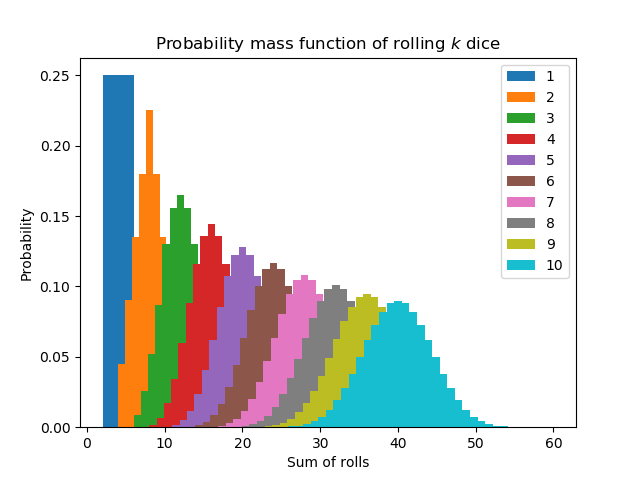
\includegraphics[scale=0.55]{pmf.png}
  \caption{PMF of every possible dice roll.}
\end{figure}

\subsection{Strategy Ignoring Feral Hogs}

Armed with our PMF, we can formulate a strategy ignoring feral hogs.
First, we define a few helper methods from Hog 
(the types in the function arguments and the -> are Python 
\href{https://docs.python.org/3/library/typing.html}{type annotations},
which are essentially comments that show type).

\begin{minted}[label=Hog functions]{python}
def free_bacon(score: int) -> int:
    return 10 - (score % 10) + score//10

def is_swap(player_score: int, opponent_score: int) -> bool:
    tens_digit = (opponent_score % 100)//10
    return abs((player_score % 10) - (opponent_score % 10)) == tens_digit

def is_feral(delta: int, k: int) -> bool: 
    return abs(delta - k) == 2
\end{minted} 

We now define a major building block of the eventual algorithm:
a function that calculates the expected value win rate after rolling \( k \) dice.
The \emphasis{expected value} is the sum of the value of each possibility times
the probability that it occurs.
Under the recursive leap of faith, we assume we have a function recur
that is able to compute the win rate given a particular delta. 
The particular pmf we use is pmf\_matrix[k - 1] because 
pmf\_matrix[0] is the distribution for 1 dice rolled, pmf\_matrix[1]
is for 2 dice rolled, and so on. denom is \( 5^k \),
because each dice has 5 options so the total number of possibilities is
\( 5^k \). \( \frac{\mathrm{pmf}[d]}{\text{denom}} \) is then the actual probability of 
a delta \( d \) occurring.
We then track two possibilities: either pig out happens or it doesn't.

The chance pig out doesn't happen is if we don't roll a 1 for all \( k \) dice.
The chance of rolling a 1 is \( \frac{1}{6} \), so the chance of not 
rolling a 1 is \( \frac{5}{6} \). Thus, the chance of not rolling a single 
1 is \( (\frac{5}{6})^k \). The chance of rolling at least 1 is then
1 minus the chance of not rolling a single 1, so \( 1 - (\frac{5}{6})^k \).
If pig out does happen, the win rate of pig out is the win rate after a delta 
of 1 (since we know our score changes by 1).
We find this win rate by calling recur on 1.

If pig out doesn't happen, we have to find what happens after multiple
possible delta values. If we roll \( k \) dice, 
the smallest delta we can get is \( 2k \) since the smallest roll is 2
and the largest delta we can get is \( 6k \) since the smallest roll is 6.
For each delta, we add up the probability of that delta occurring,
multiply by the win rate calculated by recur, and finally 
multiply by the chance that we don't pig out.

Ignore the *args in the code, they are for later use.
The backslashes in Python are line extensions, to write a particularly long line
onto multiple lines.

\begin{minted}[label=expected value]{python}
def expected_value(recur, k, *args) -> float:
    pmf, denom = pmf_matrix[k - 1], 5**k
    return (1 - (5/6)**k)*recur(1, *args) + \
               ((5/6)**k)*sum(recur(d, *args)*(pmf[d]/denom) \
                          for d in range(2*k, 6*k + 1))  
\end{minted} 

We now need to define the recur function, which takes in a delta
and returns the win rate of the resulting position.
Since our strategy ignores feral hogs, a position is defined 
by the tuple (score, opponent score). No other information is necessary.
First, we compute how the state changes after a particular delta.
Note that the scores are swapped if there is no swap,
and not swapped if there is a swap.
This is because the perspectives reverse after a move
(it is now the opponent's turn to move),
so we swap to maintain symmetry.

\begin{minted}[label=state]{python}
def state(score: int, opponent_score: int, delta: int) -> tuple:
    new, opp = score + delta, opponent_score
    return (opp, new) if not is_swap(new, opp) else (new, opp)
\end{minted}

We now suppose that our strategy is a function passed in as f.
We assume f returns a tuple of (best move, expected win rate).
Recur uses f to get the win rate of the new state,
where * is the tuple unpack (it turns a tuple into a list of arguments)
and gets [1], which is the expected win rate.
We return 1 minus that value, because the next move is from the perspective
of the opponent, so we get the win rate for the current player.

\begin{minted}[label=recur]{python}
def recur2(f, score, opponent_score, delta):
    return 1 - f(*state(score, opponent_score, delta))[1]
\end{minted} 

Given a complete definition for expected\_value,
we now create a strategy list 
which encapsulates the win rate for each possible action.
We either roll 1-10 dice, whose win rate is given by expected\_value,
or we roll 0, whose corresponding delta is computed from the free bacon rule.
In the case of free bacon, there is no probability, 
so we can call recur to directly get the next win rate. 

\begin{minted}[label=strategy]{python}
def strategy2(recur, opponent_score) -> list:
    return [(0, recur(free_bacon(opponent_score)))] + \
           [(k, expected_value(recur, k)) for k in range(1, K + 1)]
\end{minted} 

Finally, to get the best move, we take the move with the highest win rate.
We also break ties by arbitrarily picking the lower roll
(since these rolls have lower variance). 
\begin{minted}[label=best move]{python}
def best_move(strategy: list) -> tuple:
    return max(strategy, key=lambda x: (x[1], -x[0])) 
\end{minted} 

Given these methods, we construct the encapsulating strategy.
The first thing we notice is that since a position is given by (score, opponent\_score),
there are only 100*100 = 10,000 possible positions.
If we calculate the win rate for each position, then when asked for the 
same position twice we can just remember what we calculated and
return the same value. This technique is known as \emphasis{memoization}
and can be easily implemented with the lru\_cache decorator 
from the standard library functools.

The base case is if the game is over, when either my score
or the opponent score is over the GOAL\_SCORE cutoff.
In that case, we return whether the current player won or not.
If the game is not over, then we create a new recur function
that wraps the recur2 function defined earlier to only take in a argument delta.
We pass recur2 the function we are in, 
which is the recursive aspect of this algorithm.
Finally, we return the best move by computing the strategy list.

\begin{minted}[label=strategy dp]{python}
@lru_cache(maxsize=None)
def ignore_feral_dp(score, opponent_score):
    # base case: if the game is over, return whether I win or not
    if score >= GOAL_SCORE or opponent_score >= GOAL_SCORE:
        return (None, score >= GOAL_SCORE)

    recur = lambda delta: recur2(ignore_feral_dp, score, opponent_score, delta)
    return best_move(strategy2(recur, opponent_score))
\end{minted} 

As written, this is not a valid strategy since it returns 
the tuple (best move, expected win rate) for each position.
We write a simple wrapper function which returns the first element in the tuple.

\begin{minted}[label=wrapper]{python}
def ignore_feral_strategy(score, opponent_score):
    return ignore_feral_dp(score, opponent_score)[0]
\end{minted} 

I submitted this strategy early on, and found I was in a 3-way tie for first.
That seemed ridiculous to me, because I had finished the hog project 
nearly weeks in advance and had been writing my master strategy for a significant
amount ahead of time. I realized I had drastically underestimated UC Berkeley students,
and had to begin work on a new strategy.

\begin{figure}[h!]
    \centering
    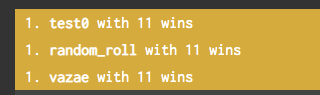
\includegraphics[scale=0.75]{tied_first.png}
    \caption{Leaderboard after this strategy (vazae was my previous team name).}
\end{figure}

The top 10 of the current leaderboard likely use a variant of this strategy. 

\newpage

\subsection{Caching Strategies}

Although this initial strategy is fast to run, the latter strategies 
start taking longer and longer, and it is convenient if one could save
the results of a strategy to a file.
Since each strategy function is a pure function of (score, opponent score),
it suffices to create an 100x100 array and store such an array to a text file.

Python defines the \href{https://docs.python.org/3/library/pickle.html}{pickle}
standard library, which can be used to dump arbitrary Python objects to a file
and load them later. We define two methods, 
load, which takes a filename and returns the object,
and dump, which takes a filename and an object and writes the object to the file.

\begin{minted}[label=pickle methods]{python}
def load(fname):
    with open(fname, "rb") as f:
        return pickle.load(f)

def dump(fname, obj):
    with open(fname, "wb") as f:
        pickle.dump(obj, f)
\end{minted} 

We are now able to dump the strategy matrix to a file for later use.
\begin{minted}[label=dump strategy to file]{python}
mat = [[final_strategy(i, j) for j in range(100)] for i in range(100)]
dump("mat.pickle", mat)
\end{minted} 

Finally, we define the final\_strategy.py file which simply loads
an existing strategy from a file. hoglib is a Python file with 
our miscellaneous utility functions, and the final\_strategy function
simply returns the corresponding element in the matrix.
\inputminted[linenos=true, fontsize=\footnotesize, label=final\_strategy.py]{Python}{programs/final_strategy.py}

If your Ok account gets hacked, the adversary will not find your actual strategy
so this doubles as a failsafe.
Also, it hides your power level.

\section{Reverse Engineering compare\_strategies.py}

During testing of this strategy, I kept getting 500 internal errors
and request limit exceeded. This annoyed me, and I decided to implement it 
myself as suggested.

Under our current framework, the sole change is to recur2.
Instead of just tracking (score, opponent score), we need to track
that along with the current turn, the change in score for the current player
(last\_delta) and the change in score for the opponent (prev\_delta).
After a particular move,
the turn just swaps from True to False, and False to True,
and one elegant way to represent that is xor with True 
(True xor True is False, and False xor True is True).
Previous delta becomes the last delta, 
and the new delta becomes the new previous delta.
However, there are 60 possible deltas, and 60*60 = 3600
so this would make our code 3600x slower.
One optimization is that we don't care if the delta is greater than 12,
because we only track these deltas to determine whether feral hogs applies,
and one can't roll more than 10 dice so the maximum delta is 12
(so that the delta is within two of the number of dice rolled).
This reduces the number of possible deltas to 13,
making the code 169x slower instead.
We add 3 to delta if the feral hogs rule applies,
but only to determine the next state as the change in the score
is calculated without the feral hogs bonus taken into account.

\begin{minted}[fontsize=\footnotesize, label=recur5]{python}
def recur5(f, score, opponent_score, turn, last_delta, prev_delta, delta, roll):
    return 1 - f(*state(score, opponent_score, delta + 3*is_feral(last_delta, roll)), 
                 turn ^ 1, prev_delta, delta if delta <= 12 else INF)
\end{minted} 

We now write the function for the comparison of two strategies, 
which we assume are defined as F1 and F2 in the global scope. 
We also define the parameter give\_all, which determines whether
all information is given to the strategies, 
or just the (score, opponent score) tuple. 
To simulate the compare\_strategies file, this parameter defaults to False.
This function has a very similar structure to that of the strategy.
We define the base case of the game being over, and if the game is not over
define a wrapper over the recur5 function that takes in a delta and the roll
which generated that delta. We then get the roll from either F1 or F2,
determining which one to use based off the current turn.
Finally, we return the win rate resulting from that action.

\begin{minted}[fontsize=\footnotesize, label=recursive comparison algorithm]{python}
@lru_cache(maxsize=None)
def server(score, opponent_score, turn, last_delta, prev_delta, give_all=False):
    if score >= GOAL_SCORE or opponent_score >= GOAL_SCORE:
        return score >= GOAL_SCORE

    state = (score, opponent_score, turn, last_delta, prev_delta)
    recur = lambda delta, roll: recur5(server, *state, delta, roll, give_all)

    f = F1 if not turn else F2
    k = f(score, opponent_score) if not give_all else \
        f(score, opponent_score, turn, last_delta, prev_delta)
    return recur(free_bacon(opponent_score), 0) if k == 0 else \
           expected_value(recur, k, k)
\end{minted} 

In order to use this comparison function, we define a wrapper compare.
compare takes in a function f which does the actual comparison, 
and two strategies s1 and s2.
It defines F1 and F2, and determines the win rate 
starting from (0, 0) with s1 going first.
If the parameter both is True, we then average the win rate 
with s1 going first with the win rate with s2 going first.
We swap the strategies to have s2 go first, and 
we negate the value to account for the change in perspective.
Before computing the new win rate, we need to first clear the cache 
since we are recomputing something different.
Finally, we return the average of the two win rates.

\begin{minted}[fontsize=\footnotesize, label=wrapper]{python}
def compare(f, s1, s2, both=True):
    global F1, F2
    F1, F2 = s1, s2
    v1 = f(0, 0, False, 0, 0)
    if both:
        f.cache_clear()
        F1, F2 = F2, F1
        v2 = 1 - f(0, 0, False, 0, 0)
    else:
        v2 = v1
    return (v1 + v2)/2 
\end{minted} 

This is a near-exact replica of the compare\_strategies.py file.

\begin{figure}[h!]
    \centering
    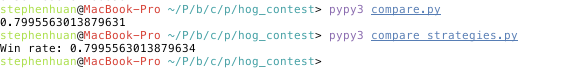
\includegraphics[scale=0.75]{compare}
    \caption{Matching the server comparison.}
\end{figure}

\subsection{Constructing a Delta Distribution}

Once I had this reverse engineered comparison file, I figured
that this could be used to my advantage.
First, we create a perfect player, which given perfect information 
of the game computes optimal play. We can test this perfect player
if we set give\_all to True.

First, instead of caching with lru\_cache as done before,
we cache with an explicit dictionary.
In order to track the possible (last delta, prev delta)
associated with each (score, opponent score, turn),
we separate the two tuples.
\begin{minted}[label=DP dictionary]{python}
dp_matrix = {(i, j, b): {} for i in range(GOAL_SCORE) \
for j in range(GOAL_SCORE) for b in range(2)}
\end{minted} 

We also modify strategy2 to be strategy5, whose only difference
is that it also passes in the roll that lead to the delta.

Finally, we define the optimal player and its wrapper function.

\begin{minted}[label=perfect DP]{python}
def perfect_dp(score, opponent_score, turn, last_delta, prev_delta):
    if score >= GOAL_SCORE or opponent_score >= GOAL_SCORE:
        return (None, score >= GOAL_SCORE)

    prefix = dp_matrix[(score, opponent_score, turn)]
    key = (last_delta, prev_delta)
    if key in prefix:
        return prefix[key] 

    state = (score, opponent_score, turn, last_delta, prev_delta)
    recur = lambda delta, roll: recur5(perfect_dp, *state, delta, roll)
    prefix[key] = best_move(strategy5(recur, opponent_score))
    return prefix[key]

def perfect_strategy(*args):
    return perfect_dp(*args)[0]
\end{minted} 

Once we have this perfect player, we modify compare to keep track of 
the frequencies of each position, using a similar explicit dictionary. 

\begin{minted}[fontsize=\footnotesize, label=record frequencies]{python}
def deltas(score, opponent_score, turn, last_delta, prev_delta, give_all=True):
    if score >= GOAL_SCORE or opponent_score >= GOAL_SCORE:
        return score >= GOAL_SCORE

    prefix = count[(score, opponent_score, turn)]
    prefix[(last_delta, prev_delta)] = prefix.get((last_delta, prev_delta), 0) + 1
    key = (score, opponent_score, turn, last_delta, prev_delta)
    if key in dp_matrix:
        return dp_matrix[key]

    recur = lambda delta, roll: recur5(deltas, *key, delta, roll, give_all)

    f = F1 if not turn else F2
    k = f(score, opponent_score) if not give_all else \
        f(score, opponent_score, turn, last_delta, prev_delta)
    dp_matrix[key] = recur(free_bacon(opponent_score), 0) if k == 0 else \
                     expected_value(recur, k, k)
    return dp_matrix[key]
\end{minted} 

This is the key insight: an approximation for the (last delta, prev delta)
distribution is given by the frequency counts generated by 
two optimal perfect-information strategies playing against each other.
Once we have this distribution, we make a new strategy accounting for it.

\newpage

\section{The Final Strategy}

Since we restructure the algorithm, we re-define recur and expected\_value.
The definitions are similar, except we introduce a new parameter feral\_bonus.

\begin{minted}[fontsize=\footnotesize, label=re-defines]{python}
@lru_cache(maxsize=None)
def final_strategy_dp(score, opponent_score, turn=False):
    if score >= GOAL_SCORE or opponent_score >= GOAL_SCORE:
        return (None, score >= GOAL_SCORE)

    def recur(delta, feral_bonus):
        return 1 - final_strategy_dp(*state(delta + feral_bonus), turn ^ 1)[1]

    def expected_value(k, feral_bonus):
        pmf, denom = pmf_matrix[k - 1], 5**k
        return (1 - (5/6)**k)*recur(1, feral_bonus) + \
                   ((5/6)**k)*sum(recur(d, feral_bonus)*pmf[d] \
                              for d in range(2*k, 6*k + 1))/denom  
\end{minted} 


We weight deltas, constructing a probability distribution where
deltas that occur more frequently are assumed to be more probable.
prob is the counts from two perfect players playing against each other,
and prob\_backup is the counts from self play.
Since what moves each strategy makes determines which positions are seen,
it is possible for a dictionary not to contain a particular delta.
First, prob is checked, then prob\_backup, and if it is in neither a 
default value of 0.25 is used.

\begin{minted}[label=weight]{python}
    def weight(deltas, turn):
        return prob[(score, opponent_score, turn)].get(deltas,
        prob_backup[(score, opponent_score, turn)].get(deltas, 0.25)) 
\end{minted} 

We then construct the delta distribution, which maps a roll
to the probability of it being feral.
We get the possible deltas through the dp\_matrix that results from 
the computation of the perfect strategy, 
and the denominator is the sum of the weights of each possible delta.
Finally, we iterate through each possible delta,
and update the probability of a certain roll being feral.
Since feral hogs applies when the roll is 2 away from the last delta,
we add a delta's weight to the roll of delta + 2 and delta - 2.

\begin{minted}[label=delta distribution]{python}
    def delta_dist(turn):
        prefix = dp_matrix[(score, opponent_score, turn)]
        # track the probability of feral hogs occuring for each dice roll.
        denom = sum(weight(deltas, turn) for deltas in prefix)
        count = {}
        for last_delta, prev_delta in prefix:
            w = weight((last_delta, prev_delta), turn)
            count[last_delta - 2] = count.get(last_delta - 2, 0) + w
            count[last_delta + 2] = count.get(last_delta + 2, 0) + w 
        return count, denom
\end{minted} 

The turn is actually also a missing piece of information, where the turn
is defined as whether you were the player who went first.
We explicitly maintain a distinction between going first and going second
by creating two delta distributions, and averaging the two.
\( p \) is then the probability that a dice roll \( k \) is feral.
feral\_value is then an extension of expected\_value, where feral\_value
computes the win rate taking into account \( p \).

\begin{minted}[label=feral\_value]{python}
    def feral_value(f, k, v):
        p = 0.5*count0.get(k, 0)/denom0 + 0.5*count1.get(k, 0)/denom1
        return p*(f(v, 3) if p > 0 else 0) + (1 - p)*(f(v, 0) if p < 1 else 0)
\end{minted} 

Given these functions, we compute the two delta distributions associated 
with going first and going second. If the denominator of a distribution is 0,
that implies the position is impossible.
If both are 0, the position is impossible so it doesn't matter what we return.
If one is impossible and the other is possible, the possible one is the 
only possibility so we copy the possible distribution into the impossible one.
Finally, if both are possible, we maintain both possibilities by doing nothing.

\begin{minted}[label=multiple distributions]{python}
    count0, denom0, count1, denom1 = *delta_dist(False), *delta_dist(True) 
    # position is impossible, default to standard dp just in case
    if denom0 == 0 and denom1 == 0:
        return final_strategy_dp1(score, opponent_score)
    # one is impossible, another isn't - copy possible into impossible
    if max(denom0, denom1) != 0 and min(denom0, denom1) == 0:
        if denom0 != 0:
            count1, denom1 = count0, denom0
        else:
            count0, denom0 = count1, denom1 
\end{minted} 

We define a strategy list and the best move.

\begin{minted}[fontsize=\footnotesize, label=strategy list]{python}
    strategy = [(0, feral_value(recur, 0, free_bacon(opponent_score)))] + \
               [(k, feral_value(expected_value, k, k)) for k in range(1, K + 1)]

    best_roll, best_ev = best_move(strategy)
\end{minted} 

\newpage

\subsection{\( \varepsilon \) Error Modeling}

We now take into account opponent errors, under a framework 
called the \emphasis{perturbed Nash equilibrium}.
The idea is the following. Suppose there is a game with this payoff matrix,
where the rows are player 1's actions and the columns are player 2's,
and each tuple represents (player 1 utility, player 2 utility).
\begin{table}[h!]
\begin{center}
\begin{tabular}{ c|c|c| }
 \multicolumn{3}{ c }{\begin{tabular}{c c c c} & A & & B \end{tabular}} \\
 \cline{2-3}
 C & -1, 1 & -1, 1  \\
 \cline{2-3}
 D & -2, 2 & -1, 1  \\
 \cline{2-3}
\end{tabular}
\end{center}
\caption{Payoff table}
\end{table}

Essentially, action A and B are the same except if player 1 plays D,
in which case A gets more utility for player 2 than B. A rational player 1
would always play C, since it avoids the risk of losing 2 when playing D.
Thus, from player 2's perspective, action A and action B are the same
since player 2 assumes that player 1 will never play D.
In the real world, however, people make mistakes.
Thus, player 2 should play A since it can only improve utility,
and in the worst case does the same as action B.
In order to model mistakes, we assume the opponent has some fixed probability
\( \varepsilon \) to make a random action.
Thus, if it is the opponent's turn, instead of returning the best expected value
directly, we return \( \varepsilon \) times the average expected value 
of the position plus \( 1 - \varepsilon \) times the best expected value.
I have \( \varepsilon = 0.01 \), so a 1\% chance to make a mistake.

\begin{minted}[label=epsilon error modeling]{python}
    # assume opponent randomly makes mistakes
    return (best_roll, (1 - EPSILON)*best_ev + \
           EPSILON*sum(x[1] for x in strategy)/len(strategy)) \
           if turn else (best_roll, best_ev)
\end{minted} 

Lastly, we define the standard wrapper.
\begin{minted}[label=wrapper]{python}
def final_strategy(score, opponent_score):
    return final_strategy_dp(score, opponent_score)[0]
\end{minted} 

\newpage

\section{Conclusion}

The assumption that the delta distribution is approximately the calls
generated by the compare function is a very primitive one, as shown 
by the very adhoc decisions working around it.
For example, 20 minutes before the deadline of the competition,
I was desperately adjusting every number in the codebase to try to get a
slight advantage over the 2\textsuperscript{nd} place at the time. 
If I had not set the final backup value to 0.25, I would have lost.

\begin{figure}[h!]
  \centering
  
\includegraphics[scale=0.75]{close}
  \caption{The current 3\textsuperscript{rd} place win rate against me, 
  minutes before the deadline.}
\end{figure}

\subsection{Future Work}

A more sophisticated approach would take into account the probability that 
each delta occurs. For example, a delta of 60 is extremely unlikely
compared to a delta of 30.
So instead of using frequency counts, the probability would be used directly.

And in general, all of these attempts to estimate a distribution for the
deltas are rooted in failure, since they are intrinsically dependent
on opponent play. To reiterate, the only truly optimal solution
is if one computed the Nash equilibrium with an algorithm like CFR.
Even if one used CFR, CFR generates a probability for each action,
not a best action. Since the Hog contest caches the function into a matrix,
a strategy is required to be a pure function.
I was assuming that the best approach would be to 
take the highest probability action for each state, but it might be better
to sample a random strategy by picking an action according to these
probabilities (e.g. if there is a 75\% chance for A and a 25\% chance for B,
instead of always picking A generate a random number and see if it is < 0.75,
and if it is, pick A and otherwise pick B).

Machine learning is of course another option, although it would be much harder
to experiment with and to prove optimality.
Dynamic programming is much more accessible, shown by the nearly 11\%
of people who used it in this year's contest. 

\newpage

\section{Appendix}
\subsection{Code}

\inputminted[linenos=true, fontsize=\tiny, label=hoglib.py]{Python}{programs/hoglib.py}
\newpage
\inputminted[linenos=true, fontsize=\tiny, label=compare.py]{Python}{programs/compare.py}
\newpage
\inputminted[linenos=true, fontsize=\scriptsize, label=final.py]{Python}{programs/final.py}
\newpage
\inputminted[linenos=true, fontsize=\footnotesize, label=final\_strategy.py]{Python}{programs/final_strategy.py}

\subsection{Team Name}

Mikoto Misaka is a character from the anime 
\href{https://myanimelist.net/anime/6213/Toaru_Kagaku_no_Railgun}
{\textit{A Certain Scientific Railgun}}.
She has the power to manipulate electricity and electromagnetic fields 
in all sorts of ways (giving her the moniker ``railgun'', as 
she is able to accelerate coins like an actual 
\href{https://en.wikipedia.org/wiki/Railgun}{railgun}).
Apparently, she is able to manipulate computers as well,
so that's why she's here.

The \href{https://toarumajutsunoindex.fandom.com/wiki/Tree_Diagram}{Tree Diagram}
is a supercomputer in this world, and I thought the name was 
particularly apropos because I was imagining tree diagrams throughout 
coding up this strategy (admittedly, ``Tree Diagram''
is a really bad name for a supercomputer).

\begin{figure}[h!]
    \centering
    \begin{subfigure}[h]{0.4 \textwidth}
      
\includegraphics[scale=0.4]{misaka}
      \caption{Mikoto Misaka}
    \end{subfigure}
    \begin{subfigure}[h]{0.4 \textwidth}
      
\includegraphics[scale=1]{Tree_Diagram}
      \caption{Tree Diagram}
    \end{subfigure}
    \caption{The team.}
\end{figure}

\printbibliography
\end{document}
